\documentclass[]{article}
\usepackage{lmodern}
\usepackage{amssymb,amsmath}
\usepackage{ifxetex,ifluatex}
\usepackage{fixltx2e} % provides \textsubscript
\ifnum 0\ifxetex 1\fi\ifluatex 1\fi=0 % if pdftex
  \usepackage[T1]{fontenc}
  \usepackage[utf8]{inputenc}
\else % if luatex or xelatex
  \ifxetex
    \usepackage{mathspec}
  \else
    \usepackage{fontspec}
  \fi
  \defaultfontfeatures{Ligatures=TeX,Scale=MatchLowercase}
\fi
% use upquote if available, for straight quotes in verbatim environments
\IfFileExists{upquote.sty}{\usepackage{upquote}}{}
% use microtype if available
\IfFileExists{microtype.sty}{%
\usepackage{microtype}
\UseMicrotypeSet[protrusion]{basicmath} % disable protrusion for tt fonts
}{}
\usepackage[margin=1in]{geometry}
\usepackage{hyperref}
\hypersetup{unicode=true,
            pdftitle={08\_EDA\_AdultCensus},
            pdfauthor={Raquel Martín - Bootcamp NEOLAND},
            pdfborder={0 0 0},
            breaklinks=true}
\urlstyle{same}  % don't use monospace font for urls
\usepackage{color}
\usepackage{fancyvrb}
\newcommand{\VerbBar}{|}
\newcommand{\VERB}{\Verb[commandchars=\\\{\}]}
\DefineVerbatimEnvironment{Highlighting}{Verbatim}{commandchars=\\\{\}}
% Add ',fontsize=\small' for more characters per line
\usepackage{framed}
\definecolor{shadecolor}{RGB}{248,248,248}
\newenvironment{Shaded}{\begin{snugshade}}{\end{snugshade}}
\newcommand{\AlertTok}[1]{\textcolor[rgb]{0.94,0.16,0.16}{#1}}
\newcommand{\AnnotationTok}[1]{\textcolor[rgb]{0.56,0.35,0.01}{\textbf{\textit{#1}}}}
\newcommand{\AttributeTok}[1]{\textcolor[rgb]{0.77,0.63,0.00}{#1}}
\newcommand{\BaseNTok}[1]{\textcolor[rgb]{0.00,0.00,0.81}{#1}}
\newcommand{\BuiltInTok}[1]{#1}
\newcommand{\CharTok}[1]{\textcolor[rgb]{0.31,0.60,0.02}{#1}}
\newcommand{\CommentTok}[1]{\textcolor[rgb]{0.56,0.35,0.01}{\textit{#1}}}
\newcommand{\CommentVarTok}[1]{\textcolor[rgb]{0.56,0.35,0.01}{\textbf{\textit{#1}}}}
\newcommand{\ConstantTok}[1]{\textcolor[rgb]{0.00,0.00,0.00}{#1}}
\newcommand{\ControlFlowTok}[1]{\textcolor[rgb]{0.13,0.29,0.53}{\textbf{#1}}}
\newcommand{\DataTypeTok}[1]{\textcolor[rgb]{0.13,0.29,0.53}{#1}}
\newcommand{\DecValTok}[1]{\textcolor[rgb]{0.00,0.00,0.81}{#1}}
\newcommand{\DocumentationTok}[1]{\textcolor[rgb]{0.56,0.35,0.01}{\textbf{\textit{#1}}}}
\newcommand{\ErrorTok}[1]{\textcolor[rgb]{0.64,0.00,0.00}{\textbf{#1}}}
\newcommand{\ExtensionTok}[1]{#1}
\newcommand{\FloatTok}[1]{\textcolor[rgb]{0.00,0.00,0.81}{#1}}
\newcommand{\FunctionTok}[1]{\textcolor[rgb]{0.00,0.00,0.00}{#1}}
\newcommand{\ImportTok}[1]{#1}
\newcommand{\InformationTok}[1]{\textcolor[rgb]{0.56,0.35,0.01}{\textbf{\textit{#1}}}}
\newcommand{\KeywordTok}[1]{\textcolor[rgb]{0.13,0.29,0.53}{\textbf{#1}}}
\newcommand{\NormalTok}[1]{#1}
\newcommand{\OperatorTok}[1]{\textcolor[rgb]{0.81,0.36,0.00}{\textbf{#1}}}
\newcommand{\OtherTok}[1]{\textcolor[rgb]{0.56,0.35,0.01}{#1}}
\newcommand{\PreprocessorTok}[1]{\textcolor[rgb]{0.56,0.35,0.01}{\textit{#1}}}
\newcommand{\RegionMarkerTok}[1]{#1}
\newcommand{\SpecialCharTok}[1]{\textcolor[rgb]{0.00,0.00,0.00}{#1}}
\newcommand{\SpecialStringTok}[1]{\textcolor[rgb]{0.31,0.60,0.02}{#1}}
\newcommand{\StringTok}[1]{\textcolor[rgb]{0.31,0.60,0.02}{#1}}
\newcommand{\VariableTok}[1]{\textcolor[rgb]{0.00,0.00,0.00}{#1}}
\newcommand{\VerbatimStringTok}[1]{\textcolor[rgb]{0.31,0.60,0.02}{#1}}
\newcommand{\WarningTok}[1]{\textcolor[rgb]{0.56,0.35,0.01}{\textbf{\textit{#1}}}}
\usepackage{graphicx,grffile}
\makeatletter
\def\maxwidth{\ifdim\Gin@nat@width>\linewidth\linewidth\else\Gin@nat@width\fi}
\def\maxheight{\ifdim\Gin@nat@height>\textheight\textheight\else\Gin@nat@height\fi}
\makeatother
% Scale images if necessary, so that they will not overflow the page
% margins by default, and it is still possible to overwrite the defaults
% using explicit options in \includegraphics[width, height, ...]{}
\setkeys{Gin}{width=\maxwidth,height=\maxheight,keepaspectratio}
\IfFileExists{parskip.sty}{%
\usepackage{parskip}
}{% else
\setlength{\parindent}{0pt}
\setlength{\parskip}{6pt plus 2pt minus 1pt}
}
\setlength{\emergencystretch}{3em}  % prevent overfull lines
\providecommand{\tightlist}{%
  \setlength{\itemsep}{0pt}\setlength{\parskip}{0pt}}
\setcounter{secnumdepth}{0}
% Redefines (sub)paragraphs to behave more like sections
\ifx\paragraph\undefined\else
\let\oldparagraph\paragraph
\renewcommand{\paragraph}[1]{\oldparagraph{#1}\mbox{}}
\fi
\ifx\subparagraph\undefined\else
\let\oldsubparagraph\subparagraph
\renewcommand{\subparagraph}[1]{\oldsubparagraph{#1}\mbox{}}
\fi

%%% Use protect on footnotes to avoid problems with footnotes in titles
\let\rmarkdownfootnote\footnote%
\def\footnote{\protect\rmarkdownfootnote}

%%% Change title format to be more compact
\usepackage{titling}

% Create subtitle command for use in maketitle
\providecommand{\subtitle}[1]{
  \posttitle{
    \begin{center}\large#1\end{center}
    }
}

\setlength{\droptitle}{-2em}

  \title{08\_EDA\_AdultCensus}
    \pretitle{\vspace{\droptitle}\centering\huge}
  \posttitle{\par}
    \author{Raquel Martín - Bootcamp NEOLAND}
    \preauthor{\centering\large\emph}
  \postauthor{\par}
      \predate{\centering\large\emph}
  \postdate{\par}
    \date{08 noviembre, 2020}


\begin{document}
\maketitle

{
\setcounter{tocdepth}{2}
\tableofcontents
}
Basado en la última práctica EDA Titanic en R Studio (el fichero
original así como el fichero HTML se encuentra en Google Drive), deben
realizar una EDA completo para este dataset:

\url{https://archive.ics.uci.edu/ml/datasets/adult}

\textbf{IMPORTANTE}: Los pasos a realizar son: - {[} {]} exploración -
{[} {]} limpieza - {[} {]} discretización

Intentar crear el output de salida en formato HTML (buscar info de
\texttt{knit} y sus dependencias)

\begin{Shaded}
\begin{Highlighting}[]
\CommentTok{\# Cargamos el juego de datos}
\NormalTok{datosAdult \textless{}{-}}\StringTok{ }\KeywordTok{read.csv}\NormalTok{(}\StringTok{\textquotesingle{}http://archive.ics.uci.edu/ml/machine{-}learning{-}databases/adult/adult.data\textquotesingle{}}\NormalTok{,}\DataTypeTok{stringsAsFactors =} \OtherTok{FALSE}\NormalTok{, }\DataTypeTok{header =} \OtherTok{FALSE}\NormalTok{)}

\CommentTok{\# Nombres de los atributos}
\KeywordTok{names}\NormalTok{(datosAdult) \textless{}{-}}\StringTok{ }\KeywordTok{c}\NormalTok{(}\StringTok{"age"}\NormalTok{,}\StringTok{"workclass"}\NormalTok{,}\StringTok{"fnlwgt"}\NormalTok{,}\StringTok{"education"}\NormalTok{,}\StringTok{"education{-}num"}\NormalTok{,}\StringTok{"marital{-}status"}\NormalTok{,}\StringTok{"occupation"}\NormalTok{,}\StringTok{"relationship"}\NormalTok{,}\StringTok{"race"}\NormalTok{,}\StringTok{"sex"}\NormalTok{,}\StringTok{"capital{-}gain"}\NormalTok{,}\StringTok{"capital{-}loss"}\NormalTok{,}\StringTok{"hour{-}per{-}week"}\NormalTok{,}\StringTok{"native{-}country"}\NormalTok{,}\StringTok{"income"}\NormalTok{)}
\end{Highlighting}
\end{Shaded}

\begin{Shaded}
\begin{Highlighting}[]
\KeywordTok{unique}\NormalTok{(datosAdult}\OperatorTok{$}\NormalTok{education)}
\end{Highlighting}
\end{Shaded}

\begin{verbatim}
##  [1] " Bachelors"    " HS-grad"      " 11th"         " Masters"     
##  [5] " 9th"          " Some-college" " Assoc-acdm"   " Assoc-voc"   
##  [9] " 7th-8th"      " Doctorate"    " Prof-school"  " 5th-6th"     
## [13] " 10th"         " 1st-4th"      " Preschool"    " 12th"
\end{verbatim}

\begin{Shaded}
\begin{Highlighting}[]
\KeywordTok{unique}\NormalTok{(datosAdult}\OperatorTok{$}\StringTok{\textasciigrave{}}\DataTypeTok{education{-}num}\StringTok{\textasciigrave{}}\NormalTok{)}
\end{Highlighting}
\end{Shaded}

\begin{verbatim}
##  [1] 13  9  7 14  5 10 12 11  4 16 15  3  6  2  1  8
\end{verbatim}

\begin{Shaded}
\begin{Highlighting}[]
\NormalTok{filas=}\StringTok{ }\KeywordTok{nrow}\NormalTok{(datosAdult)}
\NormalTok{E18=}\KeywordTok{c}\NormalTok{(}\StringTok{" Preschool"}\NormalTok{,}\StringTok{" 1st{-}4th"}\NormalTok{,}\StringTok{" 5th{-}6th"}\NormalTok{,}\StringTok{" 7th{-}8th"}\NormalTok{,}\StringTok{" 9th"}\NormalTok{,}\StringTok{" 10th"}\NormalTok{ ,}\StringTok{" 11th"}\NormalTok{,}\StringTok{" 12th"}\NormalTok{)}
\NormalTok{E912=}\KeywordTok{c}\NormalTok{(}\StringTok{" HS{-}grad"}\NormalTok{,}\StringTok{" Some{-}college"}\NormalTok{,}\StringTok{" Assoc{-}acdm"}\NormalTok{,}\StringTok{" Assoc{-}voc"}\NormalTok{)}
\NormalTok{E1316=}\KeywordTok{c}\NormalTok{(}\StringTok{" Bachelors"}\NormalTok{,}\StringTok{" Masters"}\NormalTok{ ,}\StringTok{" Prof{-}school"}\NormalTok{,}\StringTok{" Doctorate"}\NormalTok{)}
 \ControlFlowTok{for}\NormalTok{ (i }\ControlFlowTok{in} \DecValTok{1}\OperatorTok{:}\NormalTok{filas)\{}
\ControlFlowTok{if}\NormalTok{ (datosAdult}\OperatorTok{$}\NormalTok{education[i] }\OperatorTok{\%in\%}\StringTok{ }\NormalTok{E18)\{}
\NormalTok{  datosAdult}\OperatorTok{$}\NormalTok{education[i]=}\StringTok{ "E18"}
\NormalTok{\} }\ControlFlowTok{else} \ControlFlowTok{if}\NormalTok{(datosAdult}\OperatorTok{$}\NormalTok{education[i] }\OperatorTok{\%in\%}\StringTok{ }\NormalTok{E912)\{}
\NormalTok{  datosAdult}\OperatorTok{$}\NormalTok{education[i]=}\StringTok{ "E912"}
\NormalTok{\} }\ControlFlowTok{else} \ControlFlowTok{if}\NormalTok{ (datosAdult}\OperatorTok{$}\NormalTok{education[i] }\OperatorTok{\%in\%}\StringTok{ }\NormalTok{E1316)\{}
\NormalTok{  datosAdult}\OperatorTok{$}\NormalTok{education[i]=}\StringTok{ "E1316"}
\NormalTok{\}}
\NormalTok{\}}
\KeywordTok{table}\NormalTok{(datosAdult}\OperatorTok{$}\NormalTok{education)}
\end{Highlighting}
\end{Shaded}

\begin{verbatim}
## 
## E1316   E18  E912 
##  8067  4253 20241
\end{verbatim}

\hypertarget{analisis-exploratorio-de-datos---data-frame-datosadult}{%
\section{Análisis exploratorio de datos - data frame
datosAdult}\label{analisis-exploratorio-de-datos---data-frame-datosadult}}

\hypertarget{primeras-observaciones-de-las-variables---exploracion}{%
\subsection{Primeras observaciones de las variables -
exploración}\label{primeras-observaciones-de-las-variables---exploracion}}

Tras cargar el fichero, cargo la librería dplyr

\begin{Shaded}
\begin{Highlighting}[]
\KeywordTok{library}\NormalTok{(dplyr)}
\end{Highlighting}
\end{Shaded}

\begin{verbatim}
## 
## Attaching package: 'dplyr'
\end{verbatim}

\begin{verbatim}
## The following objects are masked from 'package:stats':
## 
##     filter, lag
\end{verbatim}

\begin{verbatim}
## The following objects are masked from 'package:base':
## 
##     intersect, setdiff, setequal, union
\end{verbatim}

Realizo una primera observación de las variables y de sus tipos

\begin{Shaded}
\begin{Highlighting}[]
\KeywordTok{glimpse}\NormalTok{(datosAdult)}
\end{Highlighting}
\end{Shaded}

\begin{verbatim}
## Observations: 32,561
## Variables: 15
## $ age              <int> 39, 50, 38, 53, 28, 37, 49, 52, 31, 42, 37, 3...
## $ workclass        <chr> " State-gov", " Self-emp-not-inc", " Private"...
## $ fnlwgt           <int> 77516, 83311, 215646, 234721, 338409, 284582,...
## $ education        <chr> "E1316", "E1316", "E912", "E18", "E1316", "E1...
## $ `education-num`  <int> 13, 13, 9, 7, 13, 14, 5, 9, 14, 13, 10, 13, 1...
## $ `marital-status` <chr> " Never-married", " Married-civ-spouse", " Di...
## $ occupation       <chr> " Adm-clerical", " Exec-managerial", " Handle...
## $ relationship     <chr> " Not-in-family", " Husband", " Not-in-family...
## $ race             <chr> " White", " White", " White", " Black", " Bla...
## $ sex              <chr> " Male", " Male", " Male", " Male", " Female"...
## $ `capital-gain`   <int> 2174, 0, 0, 0, 0, 0, 0, 0, 14084, 5178, 0, 0,...
## $ `capital-loss`   <int> 0, 0, 0, 0, 0, 0, 0, 0, 0, 0, 0, 0, 0, 0, 0, ...
## $ `hour-per-week`  <int> 40, 13, 40, 40, 40, 40, 16, 45, 50, 40, 80, 4...
## $ `native-country` <chr> " United-States", " United-States", " United-...
## $ income           <chr> " <=50K", " <=50K", " <=50K", " <=50K", " <=5...
\end{verbatim}

Así vemos que hay 32,561 observaciones, 15 variables de las cuales 6 son
enteros y el resto caracteres.

Vamos a ver las 6 primeras filas y las 6 últimas

\begin{Shaded}
\begin{Highlighting}[]
\KeywordTok{head}\NormalTok{(datosAdult)}
\end{Highlighting}
\end{Shaded}

\begin{verbatim}
##   age         workclass fnlwgt education education-num      marital-status
## 1  39         State-gov  77516     E1316            13       Never-married
## 2  50  Self-emp-not-inc  83311     E1316            13  Married-civ-spouse
## 3  38           Private 215646      E912             9            Divorced
## 4  53           Private 234721       E18             7  Married-civ-spouse
## 5  28           Private 338409     E1316            13  Married-civ-spouse
## 6  37           Private 284582     E1316            14  Married-civ-spouse
##           occupation   relationship   race     sex capital-gain
## 1       Adm-clerical  Not-in-family  White    Male         2174
## 2    Exec-managerial        Husband  White    Male            0
## 3  Handlers-cleaners  Not-in-family  White    Male            0
## 4  Handlers-cleaners        Husband  Black    Male            0
## 5     Prof-specialty           Wife  Black  Female            0
## 6    Exec-managerial           Wife  White  Female            0
##   capital-loss hour-per-week native-country income
## 1            0            40  United-States  <=50K
## 2            0            13  United-States  <=50K
## 3            0            40  United-States  <=50K
## 4            0            40  United-States  <=50K
## 5            0            40           Cuba  <=50K
## 6            0            40  United-States  <=50K
\end{verbatim}

\begin{Shaded}
\begin{Highlighting}[]
\KeywordTok{tail}\NormalTok{(datosAdult)}
\end{Highlighting}
\end{Shaded}

\begin{verbatim}
##       age     workclass fnlwgt education education-num      marital-status
## 32556  22       Private 310152      E912            10       Never-married
## 32557  27       Private 257302      E912            12  Married-civ-spouse
## 32558  40       Private 154374      E912             9  Married-civ-spouse
## 32559  58       Private 151910      E912             9             Widowed
## 32560  22       Private 201490      E912             9       Never-married
## 32561  52  Self-emp-inc 287927      E912             9  Married-civ-spouse
##               occupation   relationship   race     sex capital-gain
## 32556    Protective-serv  Not-in-family  White    Male            0
## 32557       Tech-support           Wife  White  Female            0
## 32558  Machine-op-inspct        Husband  White    Male            0
## 32559       Adm-clerical      Unmarried  White  Female            0
## 32560       Adm-clerical      Own-child  White    Male            0
## 32561    Exec-managerial           Wife  White  Female        15024
##       capital-loss hour-per-week native-country income
## 32556            0            40  United-States  <=50K
## 32557            0            38  United-States  <=50K
## 32558            0            40  United-States   >50K
## 32559            0            40  United-States  <=50K
## 32560            0            20  United-States  <=50K
## 32561            0            40  United-States   >50K
\end{verbatim}

Antes de comenzar, vamos a comprobar si hay algún valor NA dentro de
nuestras observaciones:

\begin{Shaded}
\begin{Highlighting}[]
\KeywordTok{any}\NormalTok{(}\KeywordTok{is.na.data.frame}\NormalTok{(datosAdult))}
\end{Highlighting}
\end{Shaded}

\begin{verbatim}
## [1] FALSE
\end{verbatim}

Como vemos que no hay ningún valor NA, procedemos a realizar un resumen
de las variables, donde podemos obesrvar cálculos como la media,
mediana, mínimo/máximo y cuartiles de nuestras variables numéricas, así
como un resumen de las variables de caracteres.

\begin{Shaded}
\begin{Highlighting}[]
\KeywordTok{summary}\NormalTok{(datosAdult)}
\end{Highlighting}
\end{Shaded}

\begin{verbatim}
##       age         workclass             fnlwgt         education        
##  Min.   :17.00   Length:32561       Min.   :  12285   Length:32561      
##  1st Qu.:28.00   Class :character   1st Qu.: 117827   Class :character  
##  Median :37.00   Mode  :character   Median : 178356   Mode  :character  
##  Mean   :38.58                      Mean   : 189778                     
##  3rd Qu.:48.00                      3rd Qu.: 237051                     
##  Max.   :90.00                      Max.   :1484705                     
##  education-num   marital-status      occupation        relationship      
##  Min.   : 1.00   Length:32561       Length:32561       Length:32561      
##  1st Qu.: 9.00   Class :character   Class :character   Class :character  
##  Median :10.00   Mode  :character   Mode  :character   Mode  :character  
##  Mean   :10.08                                                           
##  3rd Qu.:12.00                                                           
##  Max.   :16.00                                                           
##      race               sex             capital-gain    capital-loss   
##  Length:32561       Length:32561       Min.   :    0   Min.   :   0.0  
##  Class :character   Class :character   1st Qu.:    0   1st Qu.:   0.0  
##  Mode  :character   Mode  :character   Median :    0   Median :   0.0  
##                                        Mean   : 1078   Mean   :  87.3  
##                                        3rd Qu.:    0   3rd Qu.:   0.0  
##                                        Max.   :99999   Max.   :4356.0  
##  hour-per-week   native-country        income         
##  Min.   : 1.00   Length:32561       Length:32561      
##  1st Qu.:40.00   Class :character   Class :character  
##  Median :40.00   Mode  :character   Mode  :character  
##  Mean   :40.44                                        
##  3rd Qu.:45.00                                        
##  Max.   :99.00
\end{verbatim}

Y vemos los valores con unique:

\begin{Shaded}
\begin{Highlighting}[]
\KeywordTok{unique}\NormalTok{(datosAdult}\OperatorTok{$}\NormalTok{workclass)}
\end{Highlighting}
\end{Shaded}

\begin{verbatim}
## [1] " State-gov"        " Self-emp-not-inc" " Private"         
## [4] " Federal-gov"      " Local-gov"        " ?"               
## [7] " Self-emp-inc"     " Without-pay"      " Never-worked"
\end{verbatim}

\begin{Shaded}
\begin{Highlighting}[]
\KeywordTok{unique}\NormalTok{(datosAdult}\OperatorTok{$}\NormalTok{education)}
\end{Highlighting}
\end{Shaded}

\begin{verbatim}
## [1] "E1316" "E912"  "E18"
\end{verbatim}

\begin{Shaded}
\begin{Highlighting}[]
\KeywordTok{unique}\NormalTok{(datosAdult}\OperatorTok{$}\StringTok{\textasciigrave{}}\DataTypeTok{marital{-}status}\StringTok{\textasciigrave{}}\NormalTok{)}
\end{Highlighting}
\end{Shaded}

\begin{verbatim}
## [1] " Never-married"         " Married-civ-spouse"   
## [3] " Divorced"              " Married-spouse-absent"
## [5] " Separated"             " Married-AF-spouse"    
## [7] " Widowed"
\end{verbatim}

\begin{Shaded}
\begin{Highlighting}[]
\KeywordTok{unique}\NormalTok{(datosAdult}\OperatorTok{$}\NormalTok{occupation)}
\end{Highlighting}
\end{Shaded}

\begin{verbatim}
##  [1] " Adm-clerical"      " Exec-managerial"   " Handlers-cleaners"
##  [4] " Prof-specialty"    " Other-service"     " Sales"            
##  [7] " Craft-repair"      " Transport-moving"  " Farming-fishing"  
## [10] " Machine-op-inspct" " Tech-support"      " ?"                
## [13] " Protective-serv"   " Armed-Forces"      " Priv-house-serv"
\end{verbatim}

Dentro de la variable Occupation, vemos que existen valores de origen
desconocido (" ?"). Más adelante veremos el número de observaciones y
qué hacemos con ellos.

Seguimos viendo los valores de nuestras variables.

\begin{Shaded}
\begin{Highlighting}[]
\KeywordTok{unique}\NormalTok{(datosAdult}\OperatorTok{$}\NormalTok{relationship)}
\end{Highlighting}
\end{Shaded}

\begin{verbatim}
## [1] " Not-in-family"  " Husband"        " Wife"           " Own-child"     
## [5] " Unmarried"      " Other-relative"
\end{verbatim}

\begin{Shaded}
\begin{Highlighting}[]
\KeywordTok{unique}\NormalTok{(datosAdult}\OperatorTok{$}\NormalTok{race)}
\end{Highlighting}
\end{Shaded}

\begin{verbatim}
## [1] " White"              " Black"              " Asian-Pac-Islander"
## [4] " Amer-Indian-Eskimo" " Other"
\end{verbatim}

\begin{Shaded}
\begin{Highlighting}[]
\KeywordTok{unique}\NormalTok{(datosAdult}\OperatorTok{$}\NormalTok{sex)}
\end{Highlighting}
\end{Shaded}

\begin{verbatim}
## [1] " Male"   " Female"
\end{verbatim}

\begin{Shaded}
\begin{Highlighting}[]
\KeywordTok{unique}\NormalTok{(datosAdult}\OperatorTok{$}\StringTok{\textasciigrave{}}\DataTypeTok{native{-}country}\StringTok{\textasciigrave{}}\NormalTok{)}
\end{Highlighting}
\end{Shaded}

\begin{verbatim}
##  [1] " United-States"              " Cuba"                      
##  [3] " Jamaica"                    " India"                     
##  [5] " ?"                          " Mexico"                    
##  [7] " South"                      " Puerto-Rico"               
##  [9] " Honduras"                   " England"                   
## [11] " Canada"                     " Germany"                   
## [13] " Iran"                       " Philippines"               
## [15] " Italy"                      " Poland"                    
## [17] " Columbia"                   " Cambodia"                  
## [19] " Thailand"                   " Ecuador"                   
## [21] " Laos"                       " Taiwan"                    
## [23] " Haiti"                      " Portugal"                  
## [25] " Dominican-Republic"         " El-Salvador"               
## [27] " France"                     " Guatemala"                 
## [29] " China"                      " Japan"                     
## [31] " Yugoslavia"                 " Peru"                      
## [33] " Outlying-US(Guam-USVI-etc)" " Scotland"                  
## [35] " Trinadad&Tobago"            " Greece"                    
## [37] " Nicaragua"                  " Vietnam"                   
## [39] " Hong"                       " Ireland"                   
## [41] " Hungary"                    " Holand-Netherlands"
\end{verbatim}

Aquí también observamos que hay observaciones de pais desconocido.

\begin{Shaded}
\begin{Highlighting}[]
\KeywordTok{unique}\NormalTok{(datosAdult}\OperatorTok{$}\NormalTok{income)}
\end{Highlighting}
\end{Shaded}

\begin{verbatim}
## [1] " <=50K" " >50K"
\end{verbatim}

\hypertarget{limpieza-de-los-datos}{%
\subsection{Limpieza de los datos}\label{limpieza-de-los-datos}}

Calculamos las tablas de frecuencia para ver el numero de ocurrencias de
cada categoría de las variables de caracteres

\begin{Shaded}
\begin{Highlighting}[]
\KeywordTok{table}\NormalTok{(datosAdult}\OperatorTok{$}\StringTok{\textasciigrave{}}\DataTypeTok{native{-}country}\StringTok{\textasciigrave{}}\NormalTok{)}
\end{Highlighting}
\end{Shaded}

\begin{verbatim}
## 
##                           ?                    Cambodia 
##                         583                          19 
##                      Canada                       China 
##                         121                          75 
##                    Columbia                        Cuba 
##                          59                          95 
##          Dominican-Republic                     Ecuador 
##                          70                          28 
##                 El-Salvador                     England 
##                         106                          90 
##                      France                     Germany 
##                          29                         137 
##                      Greece                   Guatemala 
##                          29                          64 
##                       Haiti          Holand-Netherlands 
##                          44                           1 
##                    Honduras                        Hong 
##                          13                          20 
##                     Hungary                       India 
##                          13                         100 
##                        Iran                     Ireland 
##                          43                          24 
##                       Italy                     Jamaica 
##                          73                          81 
##                       Japan                        Laos 
##                          62                          18 
##                      Mexico                   Nicaragua 
##                         643                          34 
##  Outlying-US(Guam-USVI-etc)                        Peru 
##                          14                          31 
##                 Philippines                      Poland 
##                         198                          60 
##                    Portugal                 Puerto-Rico 
##                          37                         114 
##                    Scotland                       South 
##                          12                          80 
##                      Taiwan                    Thailand 
##                          51                          18 
##             Trinadad&Tobago               United-States 
##                          19                       29170 
##                     Vietnam                  Yugoslavia 
##                          67                          16
\end{verbatim}

Hay muchas categorías diferentes, por lo que vamos a agruparlas por
continentes para que quede más limpio.

Antes de ello, vamos a realizar un back up de nuestro data frame y
seguiremos trabajando desde allí.

\begin{Shaded}
\begin{Highlighting}[]
\NormalTok{datosAdult1 \textless{}{-}}\StringTok{ }\NormalTok{datosAdult}
\end{Highlighting}
\end{Shaded}

Para hacer la agrupación por continentes, primero creamos las variables
que contengan cada país. Como tenemos 583 observaciones que no sabemos a
qué país corresponden y además hay 80 observaciones que tampoco sabemos
a qué país pertenecen exactamente (South), vamos a agruparlas:

\begin{Shaded}
\begin{Highlighting}[]
\NormalTok{Asia \textless{}{-}}\StringTok{ }\KeywordTok{c}\NormalTok{(}\StringTok{" Cambodia"}\NormalTok{, }\StringTok{" China"}\NormalTok{, }\StringTok{" Hong"}\NormalTok{, }\StringTok{" India"}\NormalTok{, }\StringTok{" Iran"}\NormalTok{, }\StringTok{" Japan"}\NormalTok{, }\StringTok{" Laos"}\NormalTok{, }\StringTok{" Philippines"}\NormalTok{, }\StringTok{" Taiwan"}\NormalTok{, }\StringTok{" Thailand"}\NormalTok{, }\StringTok{" Vietnam"}\NormalTok{)}
\NormalTok{Nor\_America \textless{}{-}}\StringTok{ }\KeywordTok{c}\NormalTok{(}\StringTok{" Canada"}\NormalTok{, }\StringTok{" United{-}States"}\NormalTok{)}
\NormalTok{Sur\_America \textless{}{-}}\StringTok{ }\KeywordTok{c}\NormalTok{(}\StringTok{" Columbia"}\NormalTok{, }\StringTok{" Cuba"}\NormalTok{, }\StringTok{" Dominican{-}Republic"}\NormalTok{, }\StringTok{" Ecuador"}\NormalTok{, }\StringTok{" El{-}Salvador"}\NormalTok{, }\StringTok{" Guatemala"}\NormalTok{, }\StringTok{" Haiti"}\NormalTok{, }\StringTok{" Honduras"}\NormalTok{, }\StringTok{" Jamaica"}\NormalTok{, }\StringTok{" Mexico"}\NormalTok{, }\StringTok{" Nicaragua"}\NormalTok{, }\StringTok{" Outlying{-}US(Guam{-}USVI{-}etc"}\NormalTok{, }\StringTok{" Peru"}\NormalTok{, }\StringTok{" Puerto{-}Rico"}\NormalTok{, }\StringTok{" Trinidad\&Tobago"}\NormalTok{)}
\NormalTok{Europa \textless{}{-}}\KeywordTok{c}\NormalTok{(}\StringTok{" England"}\NormalTok{, }\StringTok{" France"}\NormalTok{, }\StringTok{" Germany"}\NormalTok{, }\StringTok{" Greece"}\NormalTok{, }\StringTok{" Holand{-}Netherlands"}\NormalTok{, }\StringTok{" Hungary"}\NormalTok{, }\StringTok{" Ireland"}\NormalTok{, }\StringTok{" Italy"}\NormalTok{, }\StringTok{" Poland"}\NormalTok{, }\StringTok{" Portugal"}\NormalTok{, }\StringTok{" Scotland"}\NormalTok{, }\StringTok{" Yugoslavia"}\NormalTok{)}
\NormalTok{Otros \textless{}{-}}\StringTok{ }\KeywordTok{c}\NormalTok{(}\StringTok{" South"}\NormalTok{, }\StringTok{" ?"}\NormalTok{)}
\end{Highlighting}
\end{Shaded}

Realizamos una función que agrupe los paises según el continente al que
pertenezcan según las variables que acabamos de definir:

\begin{Shaded}
\begin{Highlighting}[]
\NormalTok{continente \textless{}{-}}\ControlFlowTok{function}\NormalTok{(pais)\{}
    \ControlFlowTok{if}\NormalTok{(pais }\OperatorTok{\%in\%}\StringTok{ }\NormalTok{Asia)\{}
      \KeywordTok{return}\NormalTok{(}\StringTok{"Asia"}\NormalTok{)}
\NormalTok{    \}}\ControlFlowTok{else} \ControlFlowTok{if}\NormalTok{(pais }\OperatorTok{\%in\%}\StringTok{ }\NormalTok{Nor\_America)\{}
      \KeywordTok{return}\NormalTok{(}\StringTok{"Nor\_America"}\NormalTok{)}
\NormalTok{    \}}\ControlFlowTok{else} \ControlFlowTok{if}\NormalTok{(pais }\OperatorTok{\%in\%}\StringTok{ }\NormalTok{Sur\_America)\{}
      \KeywordTok{return}\NormalTok{(}\StringTok{"Sur\_America"}\NormalTok{)}
\NormalTok{    \}}\ControlFlowTok{else} \ControlFlowTok{if}\NormalTok{(pais }\OperatorTok{\%in\%}\StringTok{ }\NormalTok{Europa)\{}
      \KeywordTok{return}\NormalTok{(}\StringTok{"Europa"}\NormalTok{)}
\NormalTok{    \}}\ControlFlowTok{else}\NormalTok{\{}
      \KeywordTok{return}\NormalTok{(}\StringTok{"Otros"}\NormalTok{)}
\NormalTok{    \}}
\NormalTok{\}}
\end{Highlighting}
\end{Shaded}

Cambiamos la variable native-country con los datos de los continentes
que acabamos de hacer:

\begin{Shaded}
\begin{Highlighting}[]
\NormalTok{datosAdult1}\OperatorTok{$}\StringTok{\textasciigrave{}}\DataTypeTok{native{-}country}\StringTok{\textasciigrave{}}\NormalTok{\textless{}{-}}\StringTok{ }\KeywordTok{sapply}\NormalTok{(datosAdult1}\OperatorTok{$}\StringTok{\textasciigrave{}}\DataTypeTok{native{-}country}\StringTok{\textasciigrave{}}\NormalTok{, continente)}
\end{Highlighting}
\end{Shaded}

Y comprobamos que la variable se haya modificado correctamente:

\begin{Shaded}
\begin{Highlighting}[]
\KeywordTok{table}\NormalTok{(datosAdult1}\OperatorTok{$}\StringTok{\textasciigrave{}}\DataTypeTok{native{-}country}\StringTok{\textasciigrave{}}\NormalTok{)}
\end{Highlighting}
\end{Shaded}

\begin{verbatim}
## 
##        Asia      Europa Nor_America       Otros Sur_America 
##         671         521       29291         696        1382
\end{verbatim}

Tras agrupar los datos según los paises, vemos que ahora tenemos solo 5
valores distintos.

Vamos a seguir con el resto de variables.

\begin{Shaded}
\begin{Highlighting}[]
\KeywordTok{table}\NormalTok{(datosAdult1}\OperatorTok{$}\StringTok{\textasciigrave{}}\DataTypeTok{marital{-}status}\StringTok{\textasciigrave{}}\NormalTok{)}
\end{Highlighting}
\end{Shaded}

\begin{verbatim}
## 
##               Divorced      Married-AF-spouse     Married-civ-spouse 
##                   4443                     23                  14976 
##  Married-spouse-absent          Never-married              Separated 
##                    418                  10683                   1025 
##                Widowed 
##                    993
\end{verbatim}

Vemos los diferentes datos de la variable estado marital. Observamos,
por ejemplo, que diferencia entre casados con un civil, con un no civil
y casados que su pareja vive en otro lugar por trabajo
(married-af-spouse, married-civ-spouse y married-spouse-absent).
Agrupamos esos datos como casados. También vamos a diferenciar entre los
que han estado casados pero ya no lo están (divorciados, separados y
viudos) y aquellos que no han estado nunca casados.

Para ello definimos 3 variables de casado, no.casado y nunca.casado:

\begin{Shaded}
\begin{Highlighting}[]
\NormalTok{casado \textless{}{-}}\StringTok{ }\KeywordTok{c}\NormalTok{(}\StringTok{" Married{-}AF{-}spouse"}\NormalTok{, }\StringTok{" Married{-}civ{-}spouse"}\NormalTok{, }\StringTok{"Married{-}spouse{-}absent"}\NormalTok{)}
\NormalTok{no.casado \textless{}{-}}\StringTok{ }\KeywordTok{c}\NormalTok{(}\StringTok{" Divorced"}\NormalTok{, }\StringTok{" Separated"}\NormalTok{, }\StringTok{" Widowed"}\NormalTok{)}
\NormalTok{nunca.casado \textless{}{-}}\StringTok{ }\KeywordTok{c}\NormalTok{(}\StringTok{" Never{-}married"}\NormalTok{)}
\end{Highlighting}
\end{Shaded}

Realizamos una función que devuelva cada una de las variables que hemos
creado según el estado civil:

\begin{Shaded}
\begin{Highlighting}[]
\NormalTok{estado.civil \textless{}{-}}\StringTok{ }\ControlFlowTok{function}\NormalTok{(estado)\{}
  \ControlFlowTok{if}\NormalTok{(estado }\OperatorTok{\%in\%}\StringTok{ }\NormalTok{casado)\{}
    \KeywordTok{return}\NormalTok{(}\StringTok{"casado"}\NormalTok{)}
\NormalTok{  \}}\ControlFlowTok{else} \ControlFlowTok{if}\NormalTok{(estado }\OperatorTok{\%in\%}\StringTok{ }\NormalTok{no.casado)\{}
    \KeywordTok{return}\NormalTok{(}\StringTok{"no.casado"}\NormalTok{)}
\NormalTok{  \}}\ControlFlowTok{else}\NormalTok{\{}
    \KeywordTok{return}\NormalTok{(}\StringTok{"nunca.casado"}\NormalTok{)}
\NormalTok{  \}}
\NormalTok{\}}
\end{Highlighting}
\end{Shaded}

Cambiamos los datos en la variable marital-status según la función que
acabamos de hacer:

\begin{Shaded}
\begin{Highlighting}[]
\NormalTok{datosAdult1}\OperatorTok{$}\StringTok{\textasciigrave{}}\DataTypeTok{marital{-}status}\StringTok{\textasciigrave{}}\NormalTok{\textless{}{-}}\StringTok{ }\KeywordTok{sapply}\NormalTok{(datosAdult1}\OperatorTok{$}\StringTok{\textasciigrave{}}\DataTypeTok{marital{-}status}\StringTok{\textasciigrave{}}\NormalTok{, estado.civil)}
\end{Highlighting}
\end{Shaded}

Y comprobamos que se haya cambiado correctamente:

\begin{Shaded}
\begin{Highlighting}[]
\KeywordTok{table}\NormalTok{(datosAdult1}\OperatorTok{$}\StringTok{\textasciigrave{}}\DataTypeTok{marital{-}status}\StringTok{\textasciigrave{}}\NormalTok{)}
\end{Highlighting}
\end{Shaded}

\begin{verbatim}
## 
##       casado    no.casado nunca.casado 
##        14999         6461        11101
\end{verbatim}

Vamos a ver ahora la variable Education:

\begin{Shaded}
\begin{Highlighting}[]
\KeywordTok{table}\NormalTok{(datosAdult1}\OperatorTok{$}\NormalTok{education)}
\end{Highlighting}
\end{Shaded}

\begin{verbatim}
## 
## E1316   E18  E912 
##  8067  4253 20241
\end{verbatim}

Podemos observar que hay muchos tipos distintos de datos, por ello
diferenciamos según lo creado en el ejemplo del principio, adaptándolo a
nuestro df de back up en el que estamos realizando todos los cambios:

\begin{Shaded}
\begin{Highlighting}[]
\NormalTok{filas=}\StringTok{ }\KeywordTok{nrow}\NormalTok{(datosAdult1)}
\NormalTok{E18=}\KeywordTok{c}\NormalTok{(}\StringTok{" Preschool"}\NormalTok{,}\StringTok{" 1st{-}4th"}\NormalTok{,}\StringTok{" 5th{-}6th"}\NormalTok{,}\StringTok{" 7th{-}8th"}\NormalTok{,}\StringTok{" 9th"}\NormalTok{,}\StringTok{" 10th"}\NormalTok{ ,}\StringTok{" 11th"}\NormalTok{,}\StringTok{" 12th"}\NormalTok{)}
\NormalTok{E912=}\KeywordTok{c}\NormalTok{(}\StringTok{" HS{-}grad"}\NormalTok{,}\StringTok{" Some{-}college"}\NormalTok{,}\StringTok{" Assoc{-}acdm"}\NormalTok{,}\StringTok{" Assoc{-}voc"}\NormalTok{)}
\NormalTok{E1316=}\KeywordTok{c}\NormalTok{(}\StringTok{" Bachelors"}\NormalTok{,}\StringTok{" Masters"}\NormalTok{ ,}\StringTok{" Prof{-}school"}\NormalTok{,}\StringTok{" Doctorate"}\NormalTok{)}
 \ControlFlowTok{for}\NormalTok{ (i }\ControlFlowTok{in} \DecValTok{1}\OperatorTok{:}\NormalTok{filas)\{}
\ControlFlowTok{if}\NormalTok{ (datosAdult1}\OperatorTok{$}\NormalTok{education[i] }\OperatorTok{\%in\%}\StringTok{ }\NormalTok{E18)\{}
\NormalTok{  datosAdult1}\OperatorTok{$}\NormalTok{education[i]=}\StringTok{ "E18"}
\NormalTok{\} }\ControlFlowTok{else} \ControlFlowTok{if}\NormalTok{(datosAdult1}\OperatorTok{$}\NormalTok{education[i] }\OperatorTok{\%in\%}\StringTok{ }\NormalTok{E912)\{}
\NormalTok{  datosAdult1}\OperatorTok{$}\NormalTok{education[i]=}\StringTok{ "E912"}
\NormalTok{\} }\ControlFlowTok{else} \ControlFlowTok{if}\NormalTok{ (datosAdult1}\OperatorTok{$}\NormalTok{education[i] }\OperatorTok{\%in\%}\StringTok{ }\NormalTok{E1316)\{}
\NormalTok{  datosAdult1}\OperatorTok{$}\NormalTok{education[i]=}\StringTok{ "E1316"}
\NormalTok{\}}
\NormalTok{\}}
\KeywordTok{table}\NormalTok{(datosAdult1}\OperatorTok{$}\NormalTok{education)}
\end{Highlighting}
\end{Shaded}

\begin{verbatim}
## 
## E1316   E18  E912 
##  8067  4253 20241
\end{verbatim}

Ahora vamos a limpiar la variable Workclass:

\begin{Shaded}
\begin{Highlighting}[]
\KeywordTok{table}\NormalTok{(datosAdult1}\OperatorTok{$}\NormalTok{workclass)}
\end{Highlighting}
\end{Shaded}

\begin{verbatim}
## 
##                 ?       Federal-gov         Local-gov      Never-worked 
##              1836               960              2093                 7 
##           Private      Self-emp-inc  Self-emp-not-inc         State-gov 
##             22696              1116              2541              1298 
##       Without-pay 
##                14
\end{verbatim}

Vemos que hay 1836 observaciones en las que se desconoce a qué se
dedican los sujetos. Como es una cantidad elevada de momento vamos a
dejarlos como desconocidos.

Pese a que cada país tiene una legislación diferente en cuanto a tipos
de contrato, observamos que hay trabajos para el gobierno (Federal-gov,
Local-gov, State-gov), personas que trabajan con contratos de los que en
España llamamos autónomos, ya sea por su cuenta o dentro de una empresa
(Self-emp-inc y Self-emp-not-inc), personas que trabajan por cuenta
ajena (Private) y personas que o bien nunca han trabajado o no cobran
(Never-worked, Without-pay). Estos últimos casos representan solo 21
observaciones de nuestro data frame de 32.561 observaciones.

Vamos a crear nuestras variables según lo que hemos visto, agrupando por
un lado lo que conocemos como autónomos y por otro aquellos que nunca
han trabajado o que no cobran. El resto vamos a dejarlo tal y como está:

\begin{Shaded}
\begin{Highlighting}[]
\NormalTok{self.emp \textless{}{-}}\StringTok{ }\KeywordTok{c}\NormalTok{(}\StringTok{" Self{-}emp{-}inc"}\NormalTok{, }\StringTok{" Self{-}emp{-}not{-}inc"}\NormalTok{)}
\NormalTok{no.pay \textless{}{-}}\StringTok{ }\KeywordTok{c}\NormalTok{(}\StringTok{" Never{-}worked"}\NormalTok{, }\StringTok{" Without{-}pay"}\NormalTok{)}
\end{Highlighting}
\end{Shaded}

A continuación creamos una función que agrupe en categorías la variable,
solo en los casos que hemos visto:

\begin{Shaded}
\begin{Highlighting}[]
\NormalTok{trabajos \textless{}{-}}\StringTok{ }\ControlFlowTok{function}\NormalTok{(trabajo)\{}
  \ControlFlowTok{if}\NormalTok{(trabajo }\OperatorTok{\%in\%}\StringTok{ }\NormalTok{self.emp)\{}
    \KeywordTok{return}\NormalTok{(}\StringTok{" self.emp"}\NormalTok{)}
\NormalTok{  \}}\ControlFlowTok{else} \ControlFlowTok{if}\NormalTok{(trabajo }\OperatorTok{\%in\%}\StringTok{ }\NormalTok{no.pay)\{}
    \KeywordTok{return}\NormalTok{(}\StringTok{" no.pay"}\NormalTok{)}
\NormalTok{  \}}\ControlFlowTok{else}\NormalTok{\{}
    \KeywordTok{return}\NormalTok{(trabajo)}
\NormalTok{  \}}
\NormalTok{\}}
\end{Highlighting}
\end{Shaded}

Como hemos hecho con las anteriores variables, modificamos la variable
con los nuevos datos y comprobamos que se haya cambiado correctamente.

\begin{Shaded}
\begin{Highlighting}[]
\NormalTok{datosAdult1}\OperatorTok{$}\NormalTok{workclass\textless{}{-}}\StringTok{ }\KeywordTok{sapply}\NormalTok{(datosAdult1}\OperatorTok{$}\NormalTok{workclass, trabajos)}
\end{Highlighting}
\end{Shaded}

\begin{Shaded}
\begin{Highlighting}[]
\KeywordTok{table}\NormalTok{(datosAdult1}\OperatorTok{$}\NormalTok{workclass)}
\end{Highlighting}
\end{Shaded}

\begin{verbatim}
## 
##            ?  Federal-gov    Local-gov       no.pay      Private 
##         1836          960         2093           21        22696 
##     self.emp    State-gov 
##         3657         1298
\end{verbatim}

\hypertarget{discretizacion}{%
\subsection{Discretización}\label{discretizacion}}

Vamos a observar un poco más nuestras variables.

La variable ingresos Income, solo diferencia entre menor o igual de 50k,
no sabemos cuál es la moneda de referencia, y más de 50k. Vemos que el
porcentaje de menor o igual de 50k es superior al de observaciones que
cobran más de esa cantidad:

\begin{Shaded}
\begin{Highlighting}[]
\KeywordTok{round}\NormalTok{(}\KeywordTok{prop.table}\NormalTok{(}\KeywordTok{table}\NormalTok{(datosAdult1}\OperatorTok{$}\NormalTok{income))}\OperatorTok{*}\DecValTok{100}\NormalTok{, }\DecValTok{2}\NormalTok{)}
\end{Highlighting}
\end{Shaded}

\begin{verbatim}
## 
##  <=50K   >50K 
##  75.92  24.08
\end{verbatim}

Exactamente un 75.92\% de las observaciones cobran menos o igual de 50k
y un 24.08\% cobra más.

Vamos a ver por continentes, cuáles tienes mayores ingresos.

\begin{Shaded}
\begin{Highlighting}[]
\KeywordTok{table}\NormalTok{(datosAdult1}\OperatorTok{$}\StringTok{\textasciigrave{}}\DataTypeTok{native{-}country}\StringTok{\textasciigrave{}}\NormalTok{, datosAdult1}\OperatorTok{$}\NormalTok{income)}
\end{Highlighting}
\end{Shaded}

\begin{verbatim}
##              
##                <=50K  >50K
##   Asia           465   206
##   Europa         369   152
##   Nor_America  22081  7210
##   Otros          532   164
##   Sur_America   1273   109
\end{verbatim}

Y en porcentajes.

\begin{Shaded}
\begin{Highlighting}[]
\KeywordTok{round}\NormalTok{(}\KeywordTok{prop.table}\NormalTok{(}\KeywordTok{table}\NormalTok{(datosAdult1}\OperatorTok{$}\StringTok{\textasciigrave{}}\DataTypeTok{native{-}country}\StringTok{\textasciigrave{}}\NormalTok{, datosAdult1}\OperatorTok{$}\NormalTok{income))}\OperatorTok{*}\DecValTok{100}\NormalTok{,}\DecValTok{2}\NormalTok{)}
\end{Highlighting}
\end{Shaded}

\begin{verbatim}
##              
##                <=50K  >50K
##   Asia          1.43  0.63
##   Europa        1.13  0.47
##   Nor_America  67.81 22.14
##   Otros         1.63  0.50
##   Sur_America   3.91  0.33
\end{verbatim}

Vamos a realizar un filtro y quedarnos con los datos de Nor\_America
para ver allí cómo se distribuyen los ingresos. Para ello creamos un
nuevo data frame ``america'', filtrando que el continente sea
``Nor\_America''

\begin{Shaded}
\begin{Highlighting}[]
\NormalTok{america \textless{}{-}}\StringTok{ }\KeywordTok{filter}\NormalTok{(datosAdult1, }\StringTok{\textasciigrave{}}\DataTypeTok{native{-}country}\StringTok{\textasciigrave{}}\OperatorTok{==}\StringTok{"Nor\_America"}\NormalTok{)}
\end{Highlighting}
\end{Shaded}

Ahora podemos ver los ingresos de menos y de más de 50k de los países
EEUU y Canadá.

\begin{Shaded}
\begin{Highlighting}[]
\KeywordTok{table}\NormalTok{(america}\OperatorTok{$}\NormalTok{income)}
\end{Highlighting}
\end{Shaded}

\begin{verbatim}
## 
##  <=50K   >50K 
##  22081   7210
\end{verbatim}

Y ver el porcentaje de ingresos diferenciando entre hombres y mujeres.
Se aprecia que el porcentaje de hombres que viven en EEUU o Canadá y que
cobran más de 50K (20,62\%) es superior al de mujeres que cobran más de
esa cantidad (3,69\%).

\begin{Shaded}
\begin{Highlighting}[]
\KeywordTok{round}\NormalTok{(}\KeywordTok{prop.table}\NormalTok{(}\KeywordTok{table}\NormalTok{(america}\OperatorTok{$}\NormalTok{income, america}\OperatorTok{$}\NormalTok{sex))}\OperatorTok{*}\DecValTok{100}\NormalTok{,}\DecValTok{2}\NormalTok{)}
\end{Highlighting}
\end{Shaded}

\begin{verbatim}
##         
##           Female  Male
##    <=50K   29.50 45.89
##    >50K     3.69 20.92
\end{verbatim}

Hay variables que contienen muchos 0 como es el caso de capital-gain y
capital-loss. Vamos a ver cuantas de nuestras observaciones son 0 en
ambos casos.

\begin{Shaded}
\begin{Highlighting}[]
\KeywordTok{table}\NormalTok{(datosAdult1}\OperatorTok{$}\StringTok{\textasciigrave{}}\DataTypeTok{capital{-}gain}\StringTok{\textasciigrave{}}\OperatorTok{==}\DecValTok{0}\NormalTok{)}
\end{Highlighting}
\end{Shaded}

\begin{verbatim}
## 
## FALSE  TRUE 
##  2712 29849
\end{verbatim}

29,849 observaciones de capital-gain son 0.

\begin{Shaded}
\begin{Highlighting}[]
\KeywordTok{table}\NormalTok{(datosAdult1}\OperatorTok{$}\StringTok{\textasciigrave{}}\DataTypeTok{capital{-}loss}\StringTok{\textasciigrave{}}\OperatorTok{==}\DecValTok{0}\NormalTok{)}
\end{Highlighting}
\end{Shaded}

\begin{verbatim}
## 
## FALSE  TRUE 
##  1519 31042
\end{verbatim}

Y 31,042 de capital-loss también son 0. Dado que la mayor parte de estas
dos variables son 0, no vamos a tenerlas en consideración y las
eliminamos de nuestro data frame.

\begin{Shaded}
\begin{Highlighting}[]
\NormalTok{datosAdult1 \textless{}{-}}\StringTok{ }\NormalTok{datosAdult1 }\OperatorTok{\%\textgreater{}\%}\StringTok{ }\KeywordTok{select}\NormalTok{(age, workclass, fnlwgt, education, }\StringTok{\textasciigrave{}}\DataTypeTok{education{-}num}\StringTok{\textasciigrave{}}\NormalTok{, }\StringTok{\textasciigrave{}}\DataTypeTok{marital{-}status}\StringTok{\textasciigrave{}}\NormalTok{, occupation}
\NormalTok{                                      , relationship, race, sex, }\StringTok{\textasciigrave{}}\DataTypeTok{hour{-}per{-}week}\StringTok{\textasciigrave{}}\NormalTok{, }\StringTok{\textasciigrave{}}\DataTypeTok{native{-}country}\StringTok{\textasciigrave{}}\NormalTok{, income)}
\end{Highlighting}
\end{Shaded}

Comprobamos que ahora datosAdult1 tiene 13 variables en lugar de 15.

\begin{Shaded}
\begin{Highlighting}[]
\KeywordTok{dim}\NormalTok{(datosAdult1)}
\end{Highlighting}
\end{Shaded}

\begin{verbatim}
## [1] 32561    13
\end{verbatim}

Considero también que la variable relationship no tiene relevancia por
lo que también vamos a prescindir de ella.

\begin{Shaded}
\begin{Highlighting}[]
\NormalTok{datosAdult1}\OperatorTok{$}\NormalTok{relationship \textless{}{-}}\StringTok{ }\OtherTok{NULL}
\end{Highlighting}
\end{Shaded}

Vamos a ver en un gráfico los ingresos según la edad de nuestras
observaciones.

\begin{Shaded}
\begin{Highlighting}[]
\KeywordTok{library}\NormalTok{(ggplot2)}
\end{Highlighting}
\end{Shaded}

\begin{verbatim}
## Warning: package 'ggplot2' was built under R version 3.6.3
\end{verbatim}

\begin{Shaded}
\begin{Highlighting}[]
\KeywordTok{ggplot}\NormalTok{(datosAdult1) }\OperatorTok{+}\StringTok{ }\KeywordTok{aes}\NormalTok{(}\DataTypeTok{x=}\KeywordTok{as.numeric}\NormalTok{(age), }\DataTypeTok{group=}\NormalTok{ income, }\DataTypeTok{fill =}\NormalTok{ income) }\OperatorTok{+}\StringTok{ }\KeywordTok{geom\_histogram}\NormalTok{(}\DataTypeTok{binwidth =} \DecValTok{1}\NormalTok{, }\DataTypeTok{color =} \StringTok{"blue"}\NormalTok{) }\OperatorTok{+}\StringTok{ }\KeywordTok{xlab}\NormalTok{(}\StringTok{"Edad"}\NormalTok{) }\OperatorTok{+}\StringTok{ }\KeywordTok{ggtitle}\NormalTok{(}\StringTok{"Ingresos según la edad"}\NormalTok{)}
\end{Highlighting}
\end{Shaded}

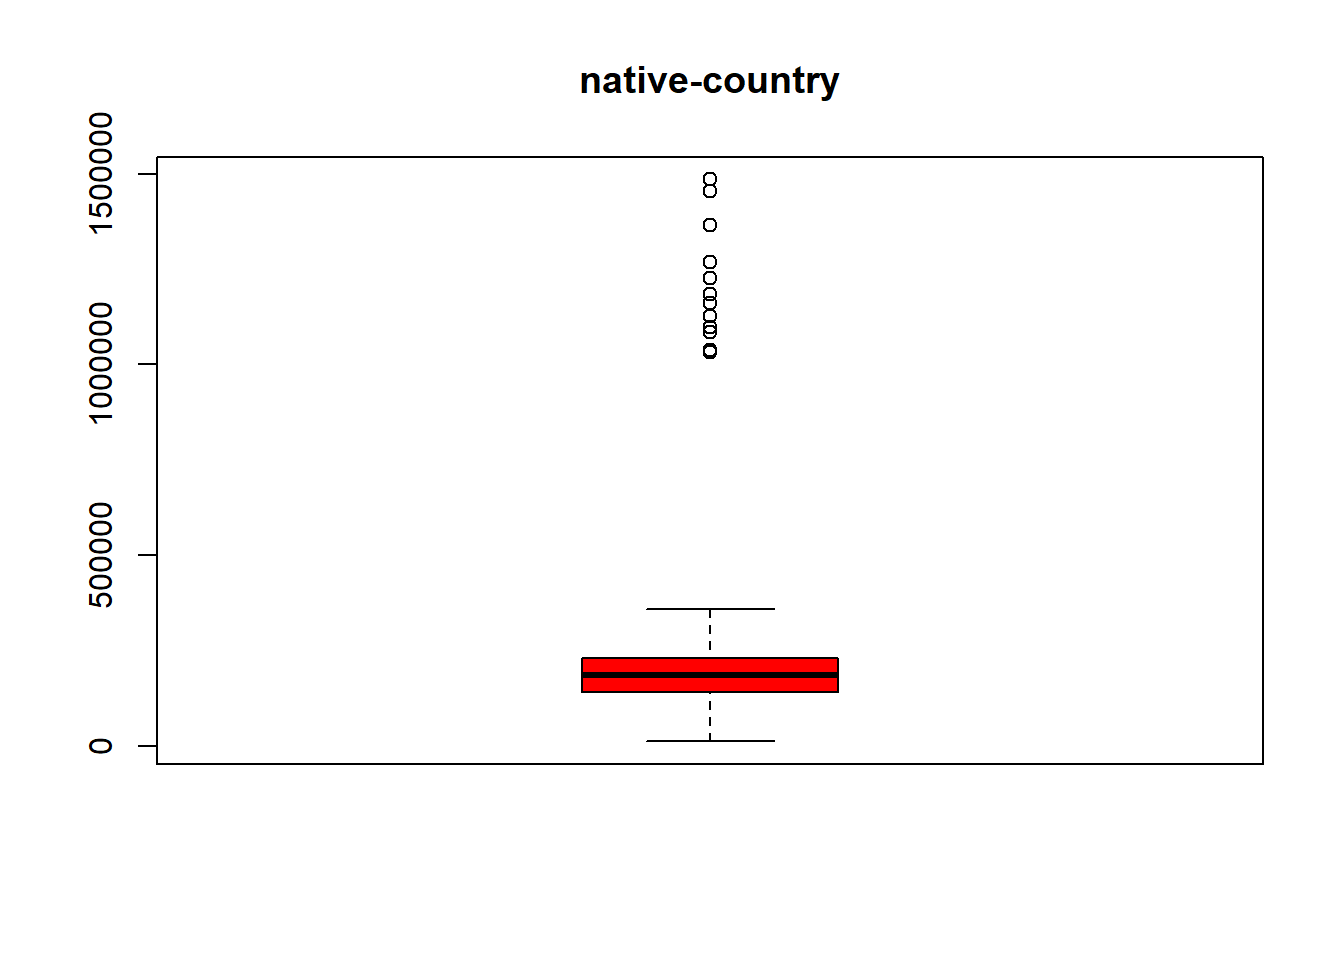
\includegraphics{01a-EDA_Adult_Raquel_files/figure-latex/unnamed-chunk-49-1.pdf}
Vamos a ver también la edad según el género.

\begin{Shaded}
\begin{Highlighting}[]
\KeywordTok{ggplot}\NormalTok{(datosAdult1) }\OperatorTok{+}\StringTok{ }\KeywordTok{aes}\NormalTok{(}\DataTypeTok{x=}\KeywordTok{as.numeric}\NormalTok{(age), }\DataTypeTok{group=}\NormalTok{ sex, }\DataTypeTok{fill =}\NormalTok{ sex) }\OperatorTok{+}\StringTok{ }\KeywordTok{geom\_histogram}\NormalTok{(}\DataTypeTok{binwidth =} \DecValTok{1}\NormalTok{, }\DataTypeTok{color =} \StringTok{"blue"}\NormalTok{) }\OperatorTok{+}\StringTok{ }\KeywordTok{xlab}\NormalTok{(}\StringTok{"Edad"}\NormalTok{) }\OperatorTok{+}\StringTok{ }\KeywordTok{ggtitle}\NormalTok{(}\StringTok{"Edad según el género"}\NormalTok{)}
\end{Highlighting}
\end{Shaded}

\includegraphics{01a-EDA_Adult_Raquel_files/figure-latex/unnamed-chunk-50-1.pdf}

Vamos a ver ahora las variables que tenemos de empleo: occupation y
workclass.

\begin{Shaded}
\begin{Highlighting}[]
\KeywordTok{table}\NormalTok{(datosAdult1}\OperatorTok{$}\NormalTok{occupation)}
\end{Highlighting}
\end{Shaded}

\begin{verbatim}
## 
##                  ?       Adm-clerical       Armed-Forces 
##               1843               3770                  9 
##       Craft-repair    Exec-managerial    Farming-fishing 
##               4099               4066                994 
##  Handlers-cleaners  Machine-op-inspct      Other-service 
##               1370               2002               3295 
##    Priv-house-serv     Prof-specialty    Protective-serv 
##                149               4140                649 
##              Sales       Tech-support   Transport-moving 
##               3650                928               1597
\end{verbatim}

\begin{Shaded}
\begin{Highlighting}[]
\KeywordTok{table}\NormalTok{(datosAdult1}\OperatorTok{$}\NormalTok{workclass)}
\end{Highlighting}
\end{Shaded}

\begin{verbatim}
## 
##            ?  Federal-gov    Local-gov       no.pay      Private 
##         1836          960         2093           21        22696 
##     self.emp    State-gov 
##         3657         1298
\end{verbatim}

La variable ocuppation tiene muchos tipos de trabajo diferentes que
pueden agruparse por categorías blue collars (operarios), white collars
(trabajos administrativos e IT), sector servicios, profesionales, ventas
y de origen desconocido (incluimos también las 9 observaciones que
trabajan en Armed-Forces por su tamaño)

Además, vamos a tratar de reducir aún más workclass unificando los
trabajos que sean del gobierno, así como a incluir los que no tienen
paga con lo de origen desconocido.

Primero creamos las variables con las nuevas categorías que hemos
elegido y asignamos cada uno de los tipos de trabajo de occupation.

\begin{Shaded}
\begin{Highlighting}[]
\NormalTok{White\_collar \textless{}{-}}\StringTok{ }\KeywordTok{c}\NormalTok{(}\StringTok{" Adm{-}clerical"}\NormalTok{, }\StringTok{" Exec{-}managerial"}\NormalTok{, }\StringTok{" Tech{-}support"}\NormalTok{)}
\NormalTok{Desconocido \textless{}{-}}\StringTok{ }\KeywordTok{c}\NormalTok{(}\StringTok{" Armed{-}Forces"}\NormalTok{, }\StringTok{" Unknown"}\NormalTok{)}
\NormalTok{Blue\_collar \textless{}{-}}\StringTok{ }\KeywordTok{c}\NormalTok{(}\StringTok{" Craft{-}repair"}\NormalTok{, }\StringTok{" Farming{-}fishing"}\NormalTok{, }\StringTok{" Handlers{-}cleaners"}\NormalTok{, }\StringTok{" Machine{-}op{-}inspct"}\NormalTok{, }\StringTok{" Transport{-}moving"}\NormalTok{)}
\NormalTok{Servicios \textless{}{-}}\StringTok{ }\KeywordTok{c}\NormalTok{(}\StringTok{" Other{-}service"}\NormalTok{, }\StringTok{" Priv{-}house{-}serv"}\NormalTok{)}
\NormalTok{Profesional \textless{}{-}}\StringTok{ }\KeywordTok{c}\NormalTok{(}\StringTok{" Prof{-}specialty"}\NormalTok{)}
\NormalTok{Ventas \textless{}{-}}\StringTok{ }\KeywordTok{c}\NormalTok{(}\StringTok{" Sales"}\NormalTok{)}
\end{Highlighting}
\end{Shaded}

Creamos una función que cambie los datos según las categorías.

\begin{Shaded}
\begin{Highlighting}[]
\NormalTok{ocupaciones \textless{}{-}}\StringTok{ }\ControlFlowTok{function}\NormalTok{(ocupacion)\{}
  \ControlFlowTok{if}\NormalTok{(ocupacion }\OperatorTok{\%in\%}\StringTok{ }\NormalTok{White\_collar)\{}
    \KeywordTok{return}\NormalTok{(}\StringTok{"White\_collar"}\NormalTok{)}
\NormalTok{  \}}\ControlFlowTok{else} \ControlFlowTok{if}\NormalTok{(ocupacion }\OperatorTok{\%in\%}\StringTok{ }\NormalTok{Ventas)\{}
    \KeywordTok{return}\NormalTok{(}\StringTok{"Sales"}\NormalTok{)}
\NormalTok{  \}}\ControlFlowTok{else} \ControlFlowTok{if}\NormalTok{(ocupacion }\OperatorTok{\%in\%}\StringTok{ }\NormalTok{Blue\_collar)\{}
    \KeywordTok{return}\NormalTok{(}\StringTok{"Blue\_collar"}\NormalTok{)}
\NormalTok{  \}}\ControlFlowTok{else} \ControlFlowTok{if}\NormalTok{(ocupacion }\OperatorTok{\%in\%}\StringTok{ }\NormalTok{Servicios)\{}
    \KeywordTok{return}\NormalTok{(}\StringTok{"Servicios"}\NormalTok{)}
\NormalTok{  \}}\ControlFlowTok{else} \ControlFlowTok{if}\NormalTok{(ocupacion }\OperatorTok{\%in\%}\StringTok{ }\NormalTok{Profesional)\{}
    \KeywordTok{return}\NormalTok{(}\StringTok{"Profesional"}\NormalTok{)}
\NormalTok{  \}}\ControlFlowTok{else}\NormalTok{\{}\KeywordTok{return}\NormalTok{(}\StringTok{"Desconocido"}\NormalTok{)\}}
\NormalTok{\}}
\end{Highlighting}
\end{Shaded}

Y modificamos nuestra variable occupation con dichas categorías.

\begin{Shaded}
\begin{Highlighting}[]
\NormalTok{datosAdult1}\OperatorTok{$}\NormalTok{occupation\textless{}{-}}\StringTok{ }\KeywordTok{sapply}\NormalTok{(datosAdult1}\OperatorTok{$}\NormalTok{occupation, ocupaciones)}
\end{Highlighting}
\end{Shaded}

\begin{Shaded}
\begin{Highlighting}[]
\KeywordTok{table}\NormalTok{(datosAdult1}\OperatorTok{$}\NormalTok{occupation)}
\end{Highlighting}
\end{Shaded}

\begin{verbatim}
## 
##  Blue_collar  Desconocido  Profesional        Sales    Servicios 
##        10062         2501         4140         3650         3444 
## White_collar 
##         8764
\end{verbatim}

Para poder hacer un gráfico con Occupation, convertimos la variable en
factor. De esta manera podemos ver visualmente

\begin{Shaded}
\begin{Highlighting}[]
\NormalTok{datosAdult1}\OperatorTok{$}\NormalTok{occupation \textless{}{-}}\StringTok{ }\KeywordTok{factor}\NormalTok{(datosAdult1}\OperatorTok{$}\NormalTok{occupation)}
\end{Highlighting}
\end{Shaded}

Contamos el número de observaciones según Occupation y los ingresos y
hacemos un nuevo data frame con esos datos.

\begin{Shaded}
\begin{Highlighting}[]
\NormalTok{count \textless{}{-}}\StringTok{ }\KeywordTok{table}\NormalTok{(datosAdult1[datosAdult1}\OperatorTok{$}\NormalTok{occupation }\OperatorTok{==}\StringTok{ "Blue\_collar"}\NormalTok{,]}\OperatorTok{$}\NormalTok{income)[}\StringTok{" \textless{}=50K"}\NormalTok{]}
\NormalTok{count \textless{}{-}}\StringTok{ }\KeywordTok{c}\NormalTok{(count, }\KeywordTok{table}\NormalTok{(datosAdult1[datosAdult1}\OperatorTok{$}\NormalTok{occupation }\OperatorTok{==}\StringTok{ "Blue\_collar"}\NormalTok{,]}\OperatorTok{$}\NormalTok{income)[}\StringTok{" \textgreater{}50K"}\NormalTok{])}
\NormalTok{count \textless{}{-}}\StringTok{ }\KeywordTok{c}\NormalTok{(count, }\KeywordTok{table}\NormalTok{(datosAdult1[datosAdult1}\OperatorTok{$}\NormalTok{occupation }\OperatorTok{==}\StringTok{ "Desconocido"}\NormalTok{,]}\OperatorTok{$}\NormalTok{income)[}\StringTok{" \textless{}=50K"}\NormalTok{])}
\NormalTok{count \textless{}{-}}\StringTok{ }\KeywordTok{c}\NormalTok{(count, }\KeywordTok{table}\NormalTok{(datosAdult1[datosAdult1}\OperatorTok{$}\NormalTok{occupation }\OperatorTok{==}\StringTok{ "Desconocido"}\NormalTok{,]}\OperatorTok{$}\NormalTok{income)[}\StringTok{" \textgreater{}50K"}\NormalTok{])}
\NormalTok{count \textless{}{-}}\StringTok{ }\KeywordTok{c}\NormalTok{(count, }\KeywordTok{table}\NormalTok{(datosAdult1[datosAdult1}\OperatorTok{$}\NormalTok{occupation }\OperatorTok{==}\StringTok{ "Profesional"}\NormalTok{,]}\OperatorTok{$}\NormalTok{income)[}\StringTok{" \textless{}=50K"}\NormalTok{])}
\NormalTok{count \textless{}{-}}\StringTok{ }\KeywordTok{c}\NormalTok{(count, }\KeywordTok{table}\NormalTok{(datosAdult1[datosAdult1}\OperatorTok{$}\NormalTok{occupation }\OperatorTok{==}\StringTok{ "Profesional"}\NormalTok{,]}\OperatorTok{$}\NormalTok{income)[}\StringTok{" \textgreater{}50K"}\NormalTok{])}
\NormalTok{count \textless{}{-}}\StringTok{ }\KeywordTok{c}\NormalTok{(count, }\KeywordTok{table}\NormalTok{(datosAdult1[datosAdult1}\OperatorTok{$}\NormalTok{occupation }\OperatorTok{==}\StringTok{ "Sales"}\NormalTok{,]}\OperatorTok{$}\NormalTok{income)[}\StringTok{" \textless{}=50K"}\NormalTok{])}
\NormalTok{count \textless{}{-}}\StringTok{ }\KeywordTok{c}\NormalTok{(count, }\KeywordTok{table}\NormalTok{(datosAdult1[datosAdult1}\OperatorTok{$}\NormalTok{occupation }\OperatorTok{==}\StringTok{ "Sales"}\NormalTok{,]}\OperatorTok{$}\NormalTok{income)[}\StringTok{" \textgreater{}50K"}\NormalTok{])}
\NormalTok{count \textless{}{-}}\StringTok{ }\KeywordTok{c}\NormalTok{(count, }\KeywordTok{table}\NormalTok{(datosAdult1[datosAdult1}\OperatorTok{$}\NormalTok{occupation }\OperatorTok{==}\StringTok{ "White\_collar"}\NormalTok{,]}\OperatorTok{$}\NormalTok{income)[}\StringTok{" \textless{}=50K"}\NormalTok{])}
\NormalTok{count \textless{}{-}}\StringTok{ }\KeywordTok{c}\NormalTok{(count, }\KeywordTok{table}\NormalTok{(datosAdult1[datosAdult1}\OperatorTok{$}\NormalTok{occupation }\OperatorTok{==}\StringTok{ "White\_collar"}\NormalTok{,]}\OperatorTok{$}\NormalTok{income)[}\StringTok{" \textgreater{}50K"}\NormalTok{])}
\NormalTok{count \textless{}{-}}\StringTok{ }\KeywordTok{c}\NormalTok{(count, }\KeywordTok{table}\NormalTok{(datosAdult1[datosAdult1}\OperatorTok{$}\NormalTok{occupation }\OperatorTok{==}\StringTok{ "Servicios"}\NormalTok{,]}\OperatorTok{$}\NormalTok{income)[}\StringTok{" \textless{}=50K"}\NormalTok{])}
\NormalTok{count \textless{}{-}}\StringTok{ }\KeywordTok{c}\NormalTok{(count, }\KeywordTok{table}\NormalTok{(datosAdult1[datosAdult1}\OperatorTok{$}\NormalTok{occupation }\OperatorTok{==}\StringTok{ "Servicios"}\NormalTok{,]}\OperatorTok{$}\NormalTok{income)[}\StringTok{" \textgreater{}50K"}\NormalTok{])}
\NormalTok{count \textless{}{-}}\StringTok{ }\KeywordTok{as.numeric}\NormalTok{(count)}
\end{Highlighting}
\end{Shaded}

\begin{Shaded}
\begin{Highlighting}[]
\NormalTok{work \textless{}{-}}\StringTok{ }\KeywordTok{rep}\NormalTok{(}\KeywordTok{levels}\NormalTok{(datosAdult1}\OperatorTok{$}\NormalTok{occupation), }\DataTypeTok{each =} \DecValTok{2}\NormalTok{)}
\NormalTok{ingresos \textless{}{-}}\StringTok{ }\KeywordTok{rep}\NormalTok{(}\KeywordTok{c}\NormalTok{(}\StringTok{" \textless{}=50K"}\NormalTok{, }\StringTok{" \textgreater{}50K"}\NormalTok{), }\DecValTok{6}\NormalTok{)}
\NormalTok{work\_ingresos \textless{}{-}}\StringTok{ }\KeywordTok{data.frame}\NormalTok{(work, ingresos, count)}
\NormalTok{work\_ingresos}
\end{Highlighting}
\end{Shaded}

\begin{verbatim}
##            work ingresos count
## 1   Blue_collar    <=50K  8362
## 2   Blue_collar     >50K  1700
## 3   Desconocido    <=50K  2098
## 4   Desconocido     >50K   403
## 5   Profesional    <=50K  2281
## 6   Profesional     >50K  1859
## 7         Sales    <=50K  2667
## 8         Sales     >50K   983
## 9     Servicios    <=50K  6006
## 10    Servicios     >50K  2758
## 11 White_collar    <=50K  3306
## 12 White_collar     >50K   138
\end{verbatim}

\begin{Shaded}
\begin{Highlighting}[]
\KeywordTok{ggplot}\NormalTok{(work\_ingresos, }\KeywordTok{aes}\NormalTok{(}\DataTypeTok{x =}\NormalTok{ work, }\DataTypeTok{y =}\NormalTok{ count, }\DataTypeTok{fill =}\NormalTok{ ingresos)) }\OperatorTok{+}\StringTok{ }\KeywordTok{geom\_bar}\NormalTok{(}\DataTypeTok{stat =} \StringTok{"identity"}\NormalTok{) }\OperatorTok{+}\StringTok{ }\KeywordTok{ggtitle}\NormalTok{(}\StringTok{"Ingresos por clase de trabajo"}\NormalTok{)}
\end{Highlighting}
\end{Shaded}

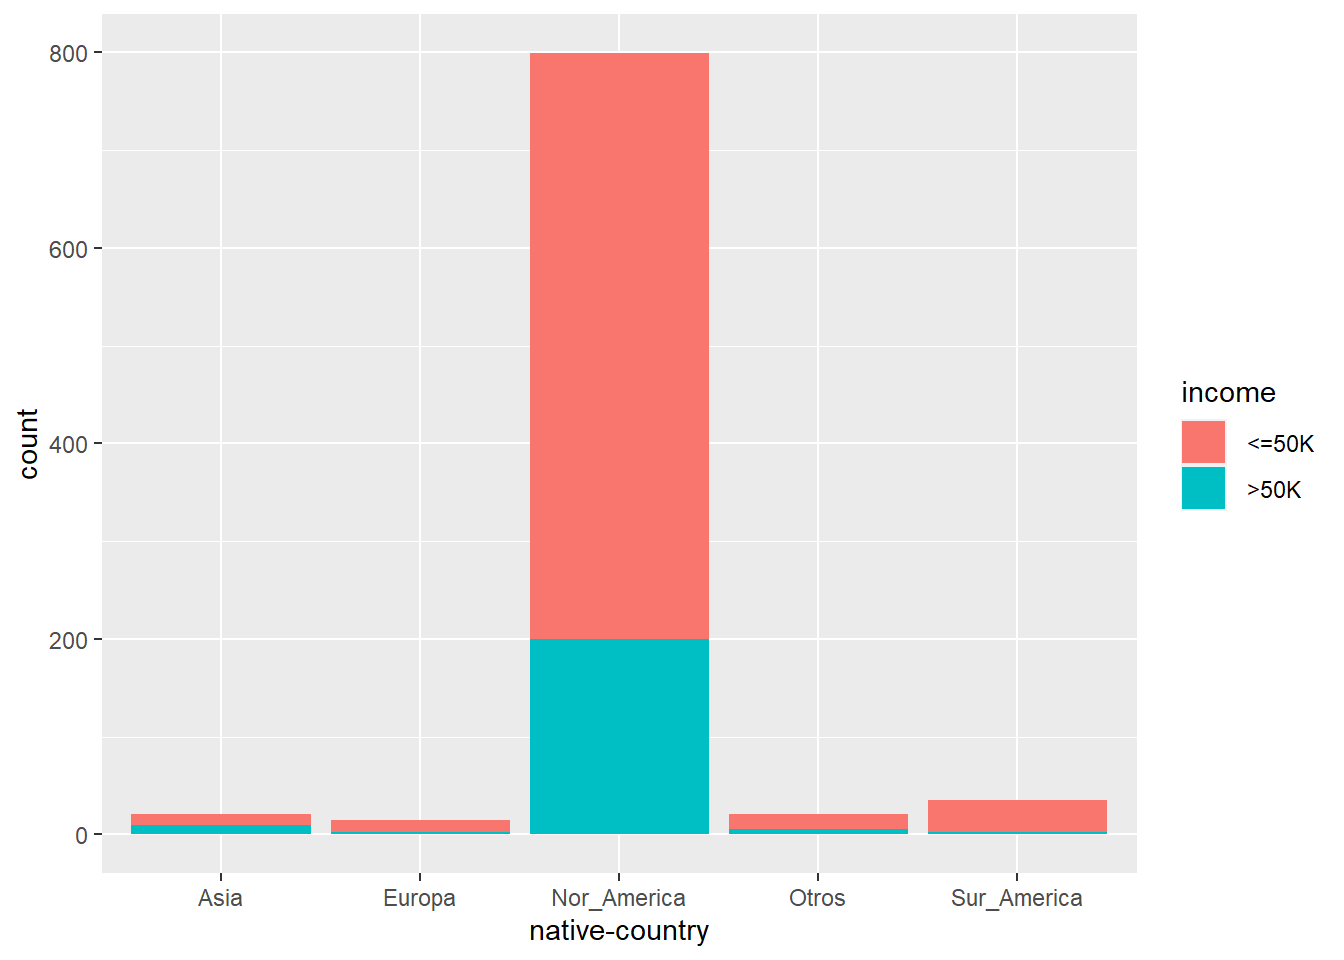
\includegraphics{01a-EDA_Adult_Raquel_files/figure-latex/unnamed-chunk-60-1.pdf}

En el gráfico podemos ver que la mayoría de blue collars u operarios
tienen unos ingresos inferiores a 50k y que dentro de los profesionales
es donde mayor igualdad de salarios hay.

Por último copiamos los datos de DatosAdult1 en DatosAdult:

\begin{Shaded}
\begin{Highlighting}[]
\NormalTok{datosAdult \textless{}{-}}\StringTok{ }\NormalTok{datosAdult1}
\end{Highlighting}
\end{Shaded}

Aquí termina nuestro análisis exploratorio de datos.


\end{document}
